%%
%% SUMMARY AND CONCLUSIONS
%%
\chapter{Summary and Conclusion}
\label{ch:summary}

\begin{fquote}[Sir Winston Churchill]Now this is not the end. It is not even the beginning of the end. But it is, perhaps, the end of the beginning. \fqsource{After Victory at El Alamein (1942)} \end{fquote} 
\begin{synopsis}
This chapter presents a summary of the work, draws conclusions from experimental results and discusses future areas of research.
\end{synopsis}

\section{Summary and Conclusions}
\label{s:summary}
This thesis studied the problem of multiresolution data in chromosomal aberration. Two datasets were available in different resolutions. In order to work with the multiple resolutions of the data, a upsampling and three different downsampling methods were proposed and their results were studied. The results were plausible and fairly consistent. The resulting data in different resolutions efficiently captures the information of data in different resolutions. Significant patterns and overall structure of the data were effectively preserved during the data transformation process. The major aim of data transformation across different resolutions was to aid in the integration of databases. Thus, after transformation to different resolutions, data was integrated for the analysis in one resolution. 

Mixture models were then applied to the data in different resolutions for all three different types of data: upsampled, downsampled, and combined. We used 10-fold cross validation approach for model selection in mixture models. The analysis of the data was performed chromosomewise in different resolutions. The results suggested that number of components required to fit the data differs across resolutions and increasing resolutions require more number of components. Furthermore, the likelihood of the model on finer resolution is poorer than that of coarse resolution although the data is the same but representation is different. Moreover, the number of components required to the fit the data is increased. The performance of the algorithm in integrated data was better than the ones performed individually in two different resolutions thus showing the importance of our data transformation process.

The trained mixture models can be used in cancer classification and clustering. The clustering results of mixture models possess high clinical significance as shown in~\cite{Myllykangas200815} and \cite{Myllykangas20067324}. Furthermore, validation by resampling showed that mixture models trained parsimoniously preserve the original structure of the data. There were only negligible discrepancies on the results of the mixture models on the data sampled from the model. The computational complexity increases with increasing resolution. Experiments with resolution 850 required approximately twice the time required for the resolution 400.

\clearpage

\section{Future Work}
\label{s:future}

\begin{figure}[h!]
\centering
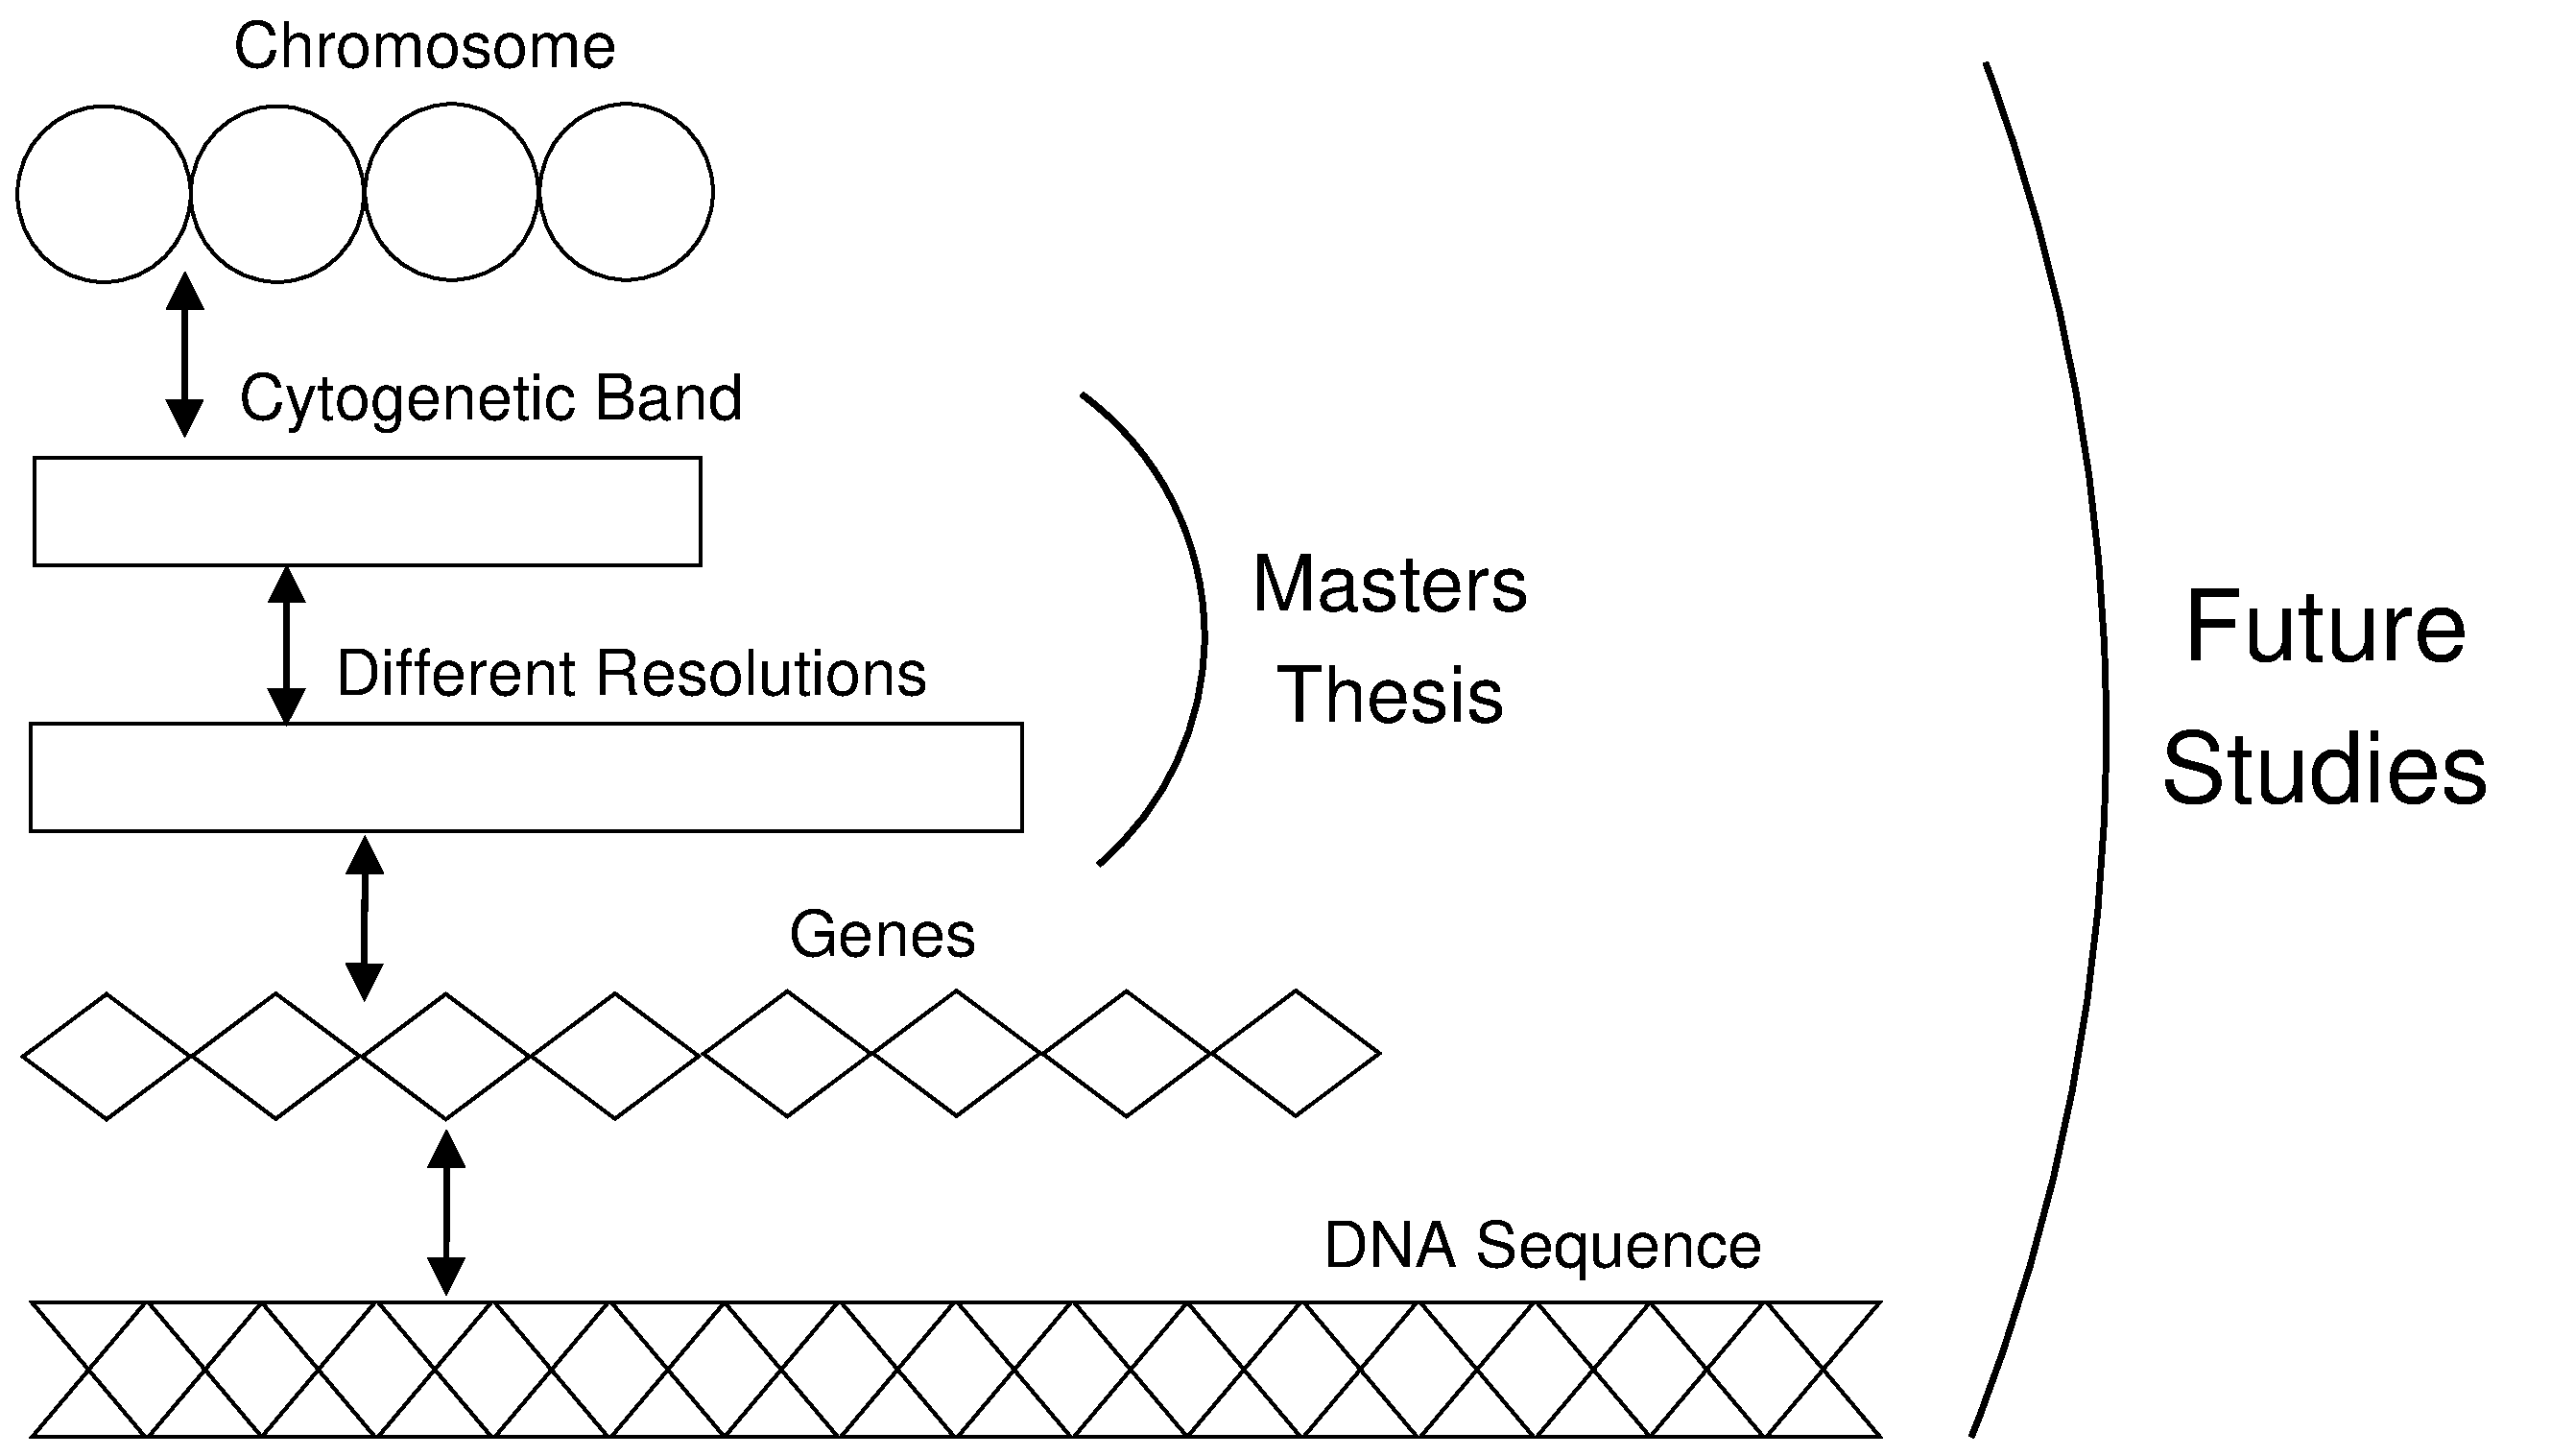
\includegraphics[width = 0.75\textwidth]{figures/problem}
\caption[Problem studied in the Master's thesis]{Schematic representation of problem studied in the Master's thesis and its seamless extension to the problem to be studied in future.} \label{Fig:problem}
\end{figure}

% As shown in Figure \ref{Fig:problem} this thesis focused on data transformation methods for changing the representation of the data in different resolution with the goal of database integration. The mixture modelling approach was then applied to the data in a single resolution. However, the field still lacks many methods and algorithms that can enhance the analysis of data in multiple resolutions without the need for transformation between different resolutions. The field seeks the  design and implementation of a multiresolution mixture model to work with multiple resolution of the data simultaneously. as shown in Figure \ref{Fig:solution}. 
% %\clearpage
% 
% \begin{figure}[h!]
% \centering
% \includegraphics[width = 0.9\textwidth]{figures/modeltry}
% \caption[Solution studied in Master's thesis]{Pictorial representation of the solution to the problem shown in Figure \ref{Fig:problem} achieved in Master's thesis and the possible solution for future studies.} \label{Fig:solution}
% \end{figure}

The multiresolution problem was studied only at chromosome level and the data transformation process was defined only in different resolutions of the chromosome. In the future work, the data transformation process can be defined until the very minute biological details such as genes and DNA sequences. Upsampling technique used in the thesis also needs further investigation and inferencing techniques can be implemented. In further work the probabilistic models, such as mixture models and probabilistic time series models, such as Hidden Markov Models(HMMs) can be extended to cope with data in multiple resolutions. 